% info-S1-intro.tex

\begin{td}[Dessins sur la plage : exécution (1)]\label{td:plage1}
On cherche à faire dessiner une figure géométrique sur la plage 
à quelqu'un qui a les yeux bandés.

Quelle figure géométrique dessine-t-on en exécutant la suite d'instructions 
ci-dessous ?
\begin{enumerate}
\item avance de 10 pas,
\item tourne à gauche d'un angle de $120^\circ$,
\item avance de 10 pas,
\item tourne à gauche d'un angle de $120^\circ$, 
\item avance de 10 pas.
\end{enumerate}
\end{td}

\begin{td}[Dessins sur la plage : conception (1)]\label{td:plage2}
Faire dessiner une spirale rectangulaire de 5 côtés, le plus petit côté
faisant 2 pas de long et chaque côté fait un pas de plus que le précédent.
\end{td}


\begin{td}[Propriétés d'un algorithme]\label{td:propPlage}
Reprendre le TD \ref{td:plage1} et illustrer la validité, la robustesse, la réutilisabilité, la
complexité et l'efficacité de l'algorithme proposé pour dessiner sur la plage.
\end{td}


\begin{td}[Unités d'information]\label{td:octets}\index[td]{unités d'information}
Combien y a-t-il d'octets dans 1 ko (kilooctet), 
1 Go (gigaoctet), 1 To (téraoctet), 1 Po (pétaoctet), 1 Eo (exaoctet),
1 Zo (zettaoctet) et 1 Yo (yottaoctet) ?
\end{td}

\begin{td}[Première utilisation de {\sc Python}]\label{td:python}\index[td]{{{\sc Python}}}
Se connecter sur un poste de travail d'une salle informatique.
\begin{enumerate}
\item Lancer {\sc Python}.
\item Utiliser {\sc Python} comme une simple calculette.
\item Quitter {\sc Python}.
\end{enumerate}
Ne pas oublier de se déconnecter du poste de travail.
\end{td}


	\begin{td}[Erreur de syntaxe en {\sc Python}]\label{td:erreur}\index[td]{{{\sc Python}}}
	On considère la session {\sc Python} suivante :\\[1mm]
	\mbox{}\hfill\begin{minipage}{7cm}\tt
	>>> x = 3\\
        >>> \ y = x\\
        \mbox{}\ \ File "<stdin>", line 1\\
        \mbox{}\ \ \ \ y = x\\
        \mbox{}\ \ \ \ \char`^\\
        SyntaxError: invalid syntax\\
        >>>
	\end{minipage}\\[1mm]
	De quelle erreur de syntaxe s'agit-il ?
	\end{td}
	
	\begin{td}[Dessins sur la plage : persévérance]\label{td:plage5}\index[td]{dessins sur la plage}
	Finir l'algorithme suivant qui cherche à dessiner un losange sur la plage.
	\begin{enumerate}
	\item avance de 10 pas,
	\item tourne à gauche d'un angle de $60^\circ$,
	\end{enumerate}
	\hspace*{0.9cm}\vdots
	\end{td}
	
	\begin{td}[Autonomie]\label{td:autonomie}\index[td]{autonomie}
	Trouver les définitions du mot autonomie et de son contraire (de son antonyme).
	\end{td}



\begin{td}[Site {\sc Web} d'Informatique S1]\label{td:site}\index[td]{site {{\sc Web}}}
Se connecter sur le site {\sc Web} du cours d'informatique S1 de l'ENIB et
vérifier que ces notes de cours sont bien disponibles sur le site
 au format {\tt pdf}.
\end{td}


\begin{td}[Exemple de contrôle d'attention (1)]\label{td:attention1}\index[td]{contrôle d'attention}
Répondre de mémoire aux questions suivantes (ie. sans rechercher les 
solutions dans les pages précédentes).
\begin{enumerate}
\item Quels sont les 3 principaux thèmes informatiques abordés ?
\item Quelles sont les 4 principales stratégies péda\-go\-giques suivies ?
\item Quelles sont les 3 principales qualités comportementales recherchées ?
\end{enumerate}
\end{td}


	\begin{td}[Exemple de contrôle de TD]\label{td:TD}\index[td]{contrôle de TD}
	Répondre aux questions du TD \ref{td:plage5}.
	\end{td}
	
	\begin{td}[Exemple de contrôle d'autoformation (1)]\label{td:bool}\index[td]{contrôle d'autoformation}
	Etablir la table de vérité du circuit logique ci-dessous où $a$, $b$
	et $c$ sont les entrées, $s$ et $t$ les sorties.\\[2mm]
	\centerline{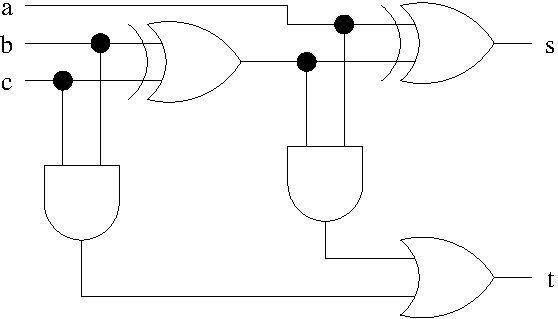
\includegraphics[width=6cm]{add3.pdf}}
	\end{td}
	
	\begin{td}[Exemple de contrôle des compétences]\label{td:competences}\index[td]{contrôle des compétences}
	Répondre aux questions du TD \ref{td:shadok} de la page \pageref{td:shadok}.
	\end{td}



\begin{td}[Nombre de contrôles]\label{td:controles}\index[td]{nombre de contrôles}
Après consultation du calendrier prévisionnel 
%de l'annexe \ref{annexe:planning} page \pageref{annexe:planning}, 
du cours d'informatique du semestre S1,
donner le nombre et le type de contrôles prévus
au calendrier du semestre.
\end{td}

	\begin{td}[Exemple de contrôle d'autoformation (2)]\label{td:negation}\index[td]{contrôle d'autoformation}
	Exprimer en la développant la négation des expressions booléennes suivantes :
	\begin{enumerate}
	\item {\tt (0 < x) and (x < 3)}
	\item {\tt (x < -2) or (x > 4)}
	\item {\tt a and (not b)}
	\item {\tt (not a) or b}
	\end{enumerate}
	\end{td}

	\begin{td}[Exemple de contrôle d'attention (2)]\label{td:attention2}\index[td]{contrôle d'attention}
	Répondre de mémoire aux questions suivantes (ie. sans rechercher les 
	solutions dans les pages précédentes).
	\begin{enumerate}
	\item Quels sont les 4 types de contrôle proposés ?
	\item Quels sont les documents que l'on peut trouver sur le site {\sc Web}
		du cours ?
	\end{enumerate}
	\end{td}

	 \begin{td}[Nombres d'exercices de TD]\label{td:exercices}\index[td]{nombres d'exercices de TD}
	 Combien d'exercices y avait-il à faire avant celui-ci ?
	 \end{td}

	\begin{td}[Environnement de travail]\label{td:labo}\index[td]{{{\sc Python}}}\index[td]{environnement de travail}
	Sur un poste de travail d'une salle informatique :
	\begin{enumerate}
	\item Quel est le type de clavier ?
	\item Comment ouvre-t-on un terminal ?
	\item Comment lance-t-on {\sc Python} ?
	\item Où sont stockés les fichiers de travail ?
	\end{enumerate}
	\end{td}

\begin{td}[QCM (1)]\label{td:qcmIntro}\index{evaluation@évaluation!contrôle d'attention}\index[td]{contrôle d'attention}
(un seul item correct par question)
\begin{enumerate}
\item L'informatique est la science
	\begin{enumerate}
	\item des dispositifs dont le fonctionnement dépend de 
		la circulation d'électrons
	\item des signaux électriques porteurs d'information ou d'énergie
	\item du traitement automatique de l'information
	\item de la commande des appareils fonctionnant sans intervention humaine
	\end{enumerate}
\item Le logiciel est
	\begin{enumerate}
	\item la mémoire de l'ordinateur
	\item le traitement automatique de l'information
	\item l'ensemble des données manipulées par les instructions
	\item un ensemble structuré d'instructions décrivant un traitement d'informations
		à faire réaliser par un matériel informatique
	\end{enumerate}
\item L'algorithmique est la science
	\begin{enumerate}
	\item du traitement automatique de l'information
	\item des algorithmes
	\item des langages de programmation
	\item des instructions
	\end{enumerate}
\item Un algorithme est
	\begin{enumerate}
	\item un ensemble de programmes remplissant une fonction déterminée,
		permettant l'accom\-plis\-se\-ment d'une tâche donnée
	\item une suite ordonnée d'instructions qui indique la démarche 
		à suivre pour résoudre une série de problèmes équivalents
	\item le nombre d'instructions élémentaires à exécuter pour
		réaliser une tâche donnée
	\item un ensemble de dispositifs physiques utilisés pour traiter
		automatiquement des informations
	\end{enumerate}
\item La validité d'un algorithme est son aptitude
	\begin{enumerate}
	\item à utiliser de manière optimale les ressources du matériel qui l'exécute
	\item à se protéger de conditions anormales d'utilisation
	\item à calculer le nombre d'instructions élémentaires nécessaires pour
		réaliser la tâche pour laquelle il a été conçu
	\item à réaliser exactement la tâche pour laquelle il a été conçu
	\end{enumerate}
\item La complexité d'un algorithme est
	\begin{enumerate}
	\item le nombre de fois où l'algorithme est utilisé dans un programme
	\item le nombre de données manipulées par les instructions de
		l'algorithme
	\item le nombre d'octets occupés en mémoire par l'algorithme
	\item le nombre d'instructions élémentaires à exécuter pour
		réaliser la tâche pour laquelle il a été conçu
	\end{enumerate}
\item Un bit est 
	\begin{enumerate}
	\item un chiffre binaire
	\item composé de 8 chiffres binaires
	\item un chiffre héxadécimal
	\item un mot d'un langage informatique
	\end{enumerate}
\item Un compilateur 
	\begin{enumerate}
	\item exécute le code source
	\item exécute le bytecode
	\item traduit un code source en code objet
	\item exécute le code objet
	\end{enumerate}
\end{enumerate}
\end{td}

\begin{td}[Puissance de calcul]\label{td:mips}\index{matériel!mips}\index[td]{puissance de calcul}
Donner l'ordre de grandeur en instructions par seconde des machines suivantes :
\begin{enumerate}
\item le premier micro-ordinateur de type PC,
\item une console de jeu actuelle,
\item un micro-ordinateur actuel,
\item {\em Deeper-Blue} : l'ordinateur qui a « battu » Kasparov aux échecs en 1997,
\item le plus puissant ordinateur actuel.
\end{enumerate}
\end{td}

\begin{td}[Stockage de données]\label{td:stock}\index[td]{stockage de données}
Donner l'ordre de grandeur en octets pour stocker en mémoire :
\begin{enumerate}
\item une page d'un livre,
\item une encyclopédie en 20 volumes,
\item une photo couleur,
\item une heure de vidéo,
\item une minute de son,
\item une heure de son.
\end{enumerate}
\end{td}

\begin{td}[Dessins sur la plage : exécution (2)]\label{td:plage3}\index[td]{dessins sur la plage}
\begin{enumerate}
\item Quelle figure géométrique dessine-t-on en exécutant la suite d'instructions 
ci-dessous ?
	\begin{enumerate}
	\item avance de 3 pas,
	\item tourne à gauche d'un angle de $90^\circ$,
	\item avance de 4 pas,
	\item rejoindre le point de départ.
	\end{enumerate}
\item Combien de pas a-t-on fait au total pour rejoindre le point de départ ?
\end{enumerate}
\end{td}

\begin{td}[Dessins sur la plage : conception (2)]\label{td:plage4}\index[td]{dessins sur la plage}
Reprendre le TD \ref{td:plage2} et illustrer la validité, la robustesse, 
la réutilisabilité, la complexité et l'efficacité de
l'algorithme proposé pour dessiner une spirale rectangulaire.
\end{td}


\begin{td}[Tracés de polygones réguliers]\label{td:tortue}\index[algo]{polygones réguliers}\index[td]{dessins sur la plage}
On cherche à faire dessiner une figure polygonale (figure \ref{fig:polygone}) 
sur la plage à quelqu'un qui a les yeux bandés.
Pour cela, on ne dispose que de 2 commandes orales :
avancer de $n$ pas en avant ($n$ est un nombre entier de pas) et 
tourner à gauche d'un angle $\theta$ (rotation sur place de $\theta$).
\begin{enumerate}
\item Faire dessiner un pentagone régulier de 10 pas de côté.
\item Faire dessiner un hexagone régulier de 10 pas de côté.
\item Faire dessiner un octogone régulier de 10 pas de côté.
\item Faire dessiner un polygone régulier de $n$ côtés de 10 pas chacun.
\end{enumerate}
\end{td}
\begin{fig}[Pentagone, hexagone, octogone]\label{fig:polygone}
\mbox{}\\
\centerline{
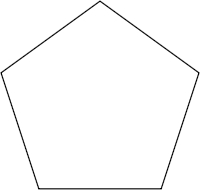
\includegraphics[width=2.5cm]{pentagone.jpg}
\hfill
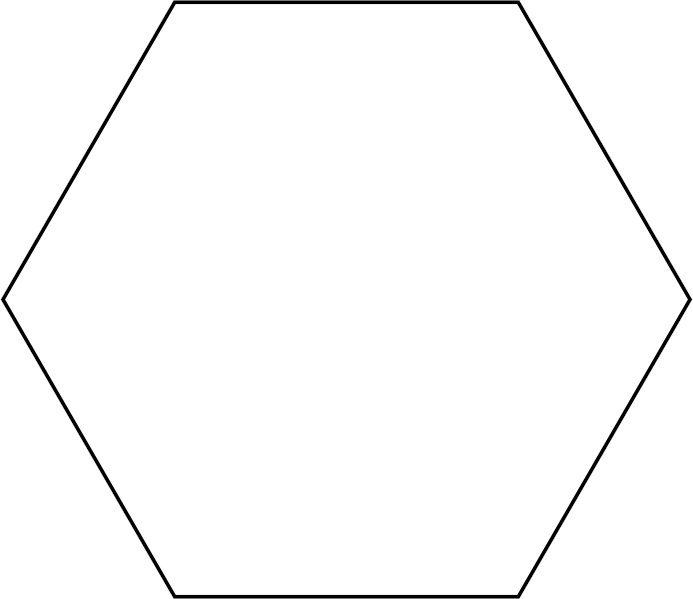
\includegraphics[width=2.5cm]{hexagone.jpg}
\hfill
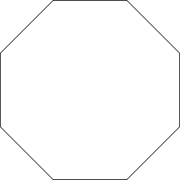
\includegraphics[width=2.5cm]{octogone.jpg}
}
\end{fig}


\begin{td}[La multiplication «~à la russe~»]\label{td:russe}\index{multiplication « à la russe »}\index[td]{multiplication « à la russe »}
La technique de multiplication dite «~à la rus\-se~» consiste à diviser par 
2 le multiplicateur (et ensuite les quotients obtenus), 
jusqu'à un quotient nul, à noter les restes,
et à multiplier parallèlement le multiplicande par 2. 
On additionne alors les multiples obtenus du multiplicande 
correspondant aux restes non nuls.

\noindent Exemple : $68 \times 123\ (= 8364)$
$$\begin{tabular}{|r|r|r|r|}
\hline
multiplicande & multiplicateur & reste      & somme partielle\\
$M \times 2$  & $m \div 2$     & $m \bmod 2$ &       \\
\hline
123  & 68 &   0   &   $(0\times 123) + 0$ \\
246  & 34 &   0   &   $(0\times 246) + 0$ \\
492  & 17 &   1   &   $(1\times 492) + 0$ \\
984  &  8 &   0   &   $(0\times 984) + 492$  \\
1968 &  4 &   0   &   $(0\times 1968) + 492$ \\
3936 &  2 &   0   &   $(0\times 3936) + 492$ \\
7872 &  1 &   1   &   $(1\times 7872) + 492$ \\
\hline
\multicolumn{3}{|r|}{$68 \times 123 =$} & 8364\\
\hline
\end{tabular}$$
\end{td}

\noindent Effectuer les multiplications suivantes selon la technique «~à la russe~».
\begin{enumerate}
\item $64 \times 96\ (= 6144)$
\item $45 \times 239\ (= 10755)$
\end{enumerate}

\begin{td}[La multiplication arabe]\label{td:ibnalbanna}
\index{multiplication arabe}\index[td]{multiplication arabe}
On consid\`ere ici le texte d'Ibn al-Banna concernant la multiplication
\`a l'aide de tableaux.

\begin{fig}[Tableau d'Ibn al-Banna]\label{fig:ibnalbanna}
\mbox{}\\
\centerline{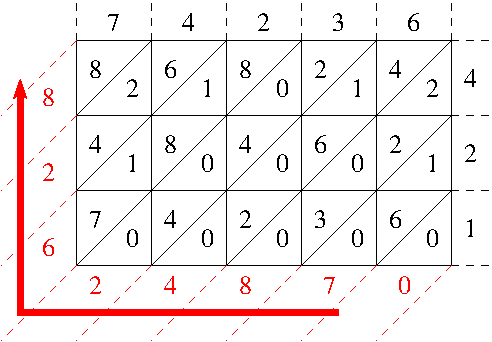
\includegraphics[width=7.5cm]{ibnalbanna.pdf}}
\end{fig}

{\footnotesize\em
« Tu construis un quadrilat\`ere que tu subdivises verticalement et
horizontalement en autant de bandes qu'il y a de positions dans les
deux nombres multipli\'es. Tu divises diagonalement les carr\'es
obtenus, \`a l'aide de diagonales allant du coin inf\'erieur gauche au
coin sup\'erieur droit (figure \ref{fig:ibnalbanna}).

Tu places le multiplicande au-dessus du quadrilat\`ere, en faisant 
correspondre chacune de ses positions \`a une colonne\footnote{L'écriture
du nombre s'effectue de droite à gauche (exemple : 352 s'écrira donc 253).}. 
Puis, tu places le multiplicateur \`a gauche ou \`a droite du quadrilat\`ere,
de telle sorte qu'il descende avec lui en faisant correspondre \'egalement 
chacune de ses positions \`a une ligne\footnote{L'écriture
du nombre s'effectue de bas en haut (exemple : {\tiny$\begin{array}{c}3\\5\\2\end{array}$} 
s'écrira donc {\tiny$\begin{array}{c}2\\5\\3\end{array}$}).}. Puis, tu multiplies, 
l'une apr\`es l'autre, chacune des positions du multiplicande du carr\'e 
par toutes les positions du multiplicateur, et tu poses le r\'esultat 
partiel correspondant \`a chaque position dans le carr\'e o\`u se coupent 
respectivement leur colonne et leur ligne, en pla\c{c}ant les unit\'es 
au-dessus de la diagonale et les dizaines en dessous. Puis, tu
commences \`a additionner, en partant du coin sup\'erieur gauche :
tu additionnes ce qui est entre les diagonales, sans effacer, 
en pla\c{c}ant chaque nombre dans sa position, en transf\'erant 
les dizaines de chaque somme partielle \`a la diagonale suivante et
en les ajoutant \`a ce qui y figure. 

La somme que tu obtiendras sera le r\'esultat. »}

\noindent En utilisant la m\'ethode du tableau d'Ibn al-Banna, calculer $63247\times124$ 
($= 7842628$).
\end{td}

\begin{td}[La division chinoise]\label{td:boulier}
\index{division chinoise}\index[td]{division chinoise}
Dans sa version actuelle, le boulier chinois se compose d'un nombre variable de tringles
serties dans un cadre rectangulaire. Sur chacune de ces tringles, deux étages de boules
séparées par une barre transversale peuvent coulisser librement (figure \ref{fig:boulier}).
La notation des nombres repose sur le principe de la numération de position : chacune
des 2 boules du haut vaut 5 unités et chacune des 5 boules du bas vaut 1 unité. Seules
comptent les boules situées dans la région transversale.

Il existe des règles spéciales de division pour chaque diviseur de 1 à 9.
On consid\`ere ici les 7 r\`egles de division par 7 (figure \ref{fig:div7}) :

\noindent\begin{minipage}[t]{7.5cm}\footnotesize
\begin{enumerate}
\item {\em «~qi-yi xia jia san~»} : 7-1 ? ajouter 3 en dessous !
\item {\em «~qi-er xia jia liu~»} : 7-2 ? ajouter 6 en dessous !
\item {\em «~qi-san si sheng er~»} : 7-3 ? 4 reste 2 !
\end{enumerate}
\end{minipage}\hfill
\begin{minipage}[t]{7.5cm}\footnotesize
\begin{enumerate}\setcounter{enumi}{3}
\item {\em «~qi-si wu sheng wu~»} : 7-4 ? 5 reste 5 !
\item {\em «~qi-wu qi sheng yi~»} : 7-5 ? 7 reste 1 !
\item {\em «~qi-liu ba sheng si~»} : 7-6 ? 8 reste 4 !
\item {\em «~feng-qi jin yi~»} : 7-7 ? 1 monté !
\end{enumerate}
\end{minipage}

\begin{fig}[Boulier chinois]\label{fig:boulier}
\mbox{}\\
\centerline{\em
8017 :
\begin{minipage}{5cm}
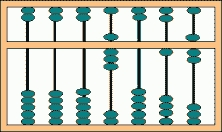
\includegraphics[width=5cm]{boulier.jpg}
\end{minipage}}
\end{fig}

\begin{fig}[Règles de la division par 7]\label{fig:div7}
\mbox{}\\
\centerline{\em\begin{tabular}[t]{|c|c|c|}
\hline
Règle & Avant & Après \\
\hline
\hline
7-1   & 
\begin{tabular}{ccccc}
1 & \makebox[0.5mm]{} & 0 & 0 & 0 \\
\hline
2 & & 0 & 1 & 0
\end{tabular} &
\begin{tabular}{ccccc}
1 & \makebox[0.5mm]{} & 0 & 0 & 0 \\
\hline
2 & & 0 & 1 & 3
\end{tabular} \\
\hline
\hline
7-2   & 
\begin{tabular}{ccccc}
1 & \makebox[0.5mm]{} & 0 & 0 & 0 \\
\hline
2 & & 0 & 2 & 0
\end{tabular} &
\begin{tabular}{ccccc}
1 & \makebox[0.5mm]{} & 0 & 0 & 1 \\
\hline
2 & & 0 & 2 & 1
\end{tabular} \\
\hline
\hline
7-3   & 
\begin{tabular}{ccccc}
1 & \makebox[0.5mm]{} & 0 & 0 & 0 \\
\hline
2 & & 0 & 3 & 0
\end{tabular} &
\begin{tabular}{ccccc}
1 & \makebox[0.5mm]{} & 0 & 0 & 0 \\
\hline
2 & & 0 & 4 & 2
\end{tabular} \\
\hline
\hline
7-4   & 
\begin{tabular}{ccccc}
1 & \makebox[0.5mm]{} & 0 & 0 & 0 \\
\hline
2 & & 0 & 4 & 0
\end{tabular} &
\begin{tabular}{ccccc}
1 & \makebox[0.5mm]{} & 0 & 1 & 1 \\
\hline
2 & & 0 & 0 & 0
\end{tabular} \\
\hline
\end{tabular}
\hspace*{2mm}
\begin{tabular}[t]{|c|c|c|}
\hline
Règle & Avant & Après \\
\hline
\hline
7-5   & 
\begin{tabular}{ccccc}
1 & \makebox[0.5mm]{} & 0 & 1 & 0 \\
\hline
2 & & 0 & 0 & 0
\end{tabular} &
\begin{tabular}{ccccc}
1 & \makebox[0.5mm]{} & 0 & 1 & 0 \\
\hline
2 & & 0 & 2 & 1
\end{tabular} \\
\hline
\hline
7-6   & 
\begin{tabular}{ccccc}
1 & \makebox[0.5mm]{} & 0 & 1 & 0 \\
\hline
2 & & 0 & 1 & 0
\end{tabular} &
\begin{tabular}{ccccc}
1 & \makebox[0.5mm]{} & 0 & 1 & 0 \\
\hline
2 & & 0 & 3 & 4
\end{tabular} \\
\hline
\hline
7-7   & 
\begin{tabular}{ccccc}
1 & \makebox[0.5mm]{} & 0 & 1 & 0 \\
\hline
2 & & 0 & 2 & 0
\end{tabular} &
\begin{tabular}{ccccc}
1 & \makebox[0.5mm]{} & 0 & 0 & 0 \\
\hline
2 & & 1 & 0 & 0
\end{tabular} \\
\hline
\end{tabular}}
\end{fig}
Ces règles ne sont pas des règles logiques, 
mais de simples procédés mnémotechniques
indiquant ce qu'il convient de faire selon la situation. Leur énoncé débute par le
rappel du diviseur, ici 7, et se poursuit par l'énoncé du dividende, par exemple 3 :
7-3. Le reste de la règle indique quelles manipulations effectuées, ajouts ou retraits
de boules. Il faut également savoir que le dividende étant posé sur le boulier, on doit
appliquer les règles aux chiffres successifs du dividende, en commençant par celui dont
l'ordre est le plus élevé.
«~ajouter en dessous~» veut dire «~mettre des boules au rang 
immédiatement inférieur (à droite) au rang considéré~» et «~monter~» veut dire «~mettre des boules
au rang immédiatement supérieur (à gauche) au rang considéré~».


Pour effectuer la division d'un nombre par 7, on pose le dividende à droite sur le
boulier et le diviseur (7) à gauche. On opère sur les chiffres successifs du dividende
en commençant par celui d'ordre le plus élevé (le plus à gauche). Les règles
précédemment énoncées sont appliquées systématiquement.

Utiliser un boulier chinois pour diviser 1234 par 7 ($1234 = 176\times 7 + 2$).

\centerline{\begin{tabular}{cccccc}
1 & \makebox[1mm]{} & 0 & 0 & 0 & 0 \\
\hline
2 & & 1 & 2 & 3 & 4
\end{tabular}
$\rightarrow$
\begin{tabular}{cccccc}
1 & \makebox[1mm]{} & 0 & 1 & 1 & 0 \\
\hline
2 & & 1 & 2 & 1 & 2
\end{tabular}}
\end{td}

\begin{td}[Le calcul Shadok]\label{td:shadok}\index{calcul {{\sc Shadok}}}\index[td]{calcul {{\sc Shadok}}}
Les cerveaux des Shadoks avaient une capacité tout à fait limitée.
Ils ne comportaient en tout que 4 cases.
Comme ils n'avaient que 4 cases, évidemment les Shadoks ne connaissaient 
pas plus de 4 mots :  {\sc ga, bu, zo et meu} (figure \ref{fig:bdShadok}).
\begin{fig}[Les Shadoks : {\sc ga} {\sc bu} {\sc zo} {\sc meu}]\label{fig:bdShadok}
\mbox{}\\
\centerline{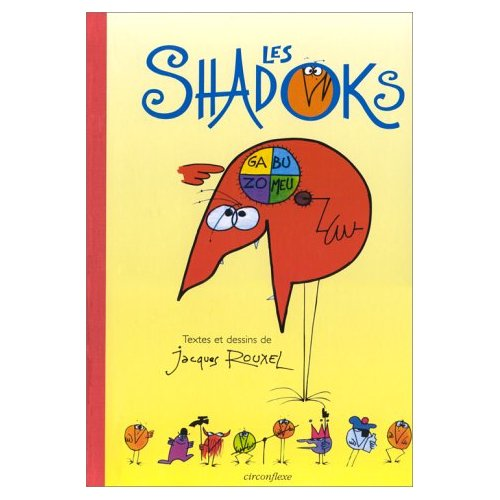
\includegraphics[width=7cm]{bdShadok.jpg}}
\end{fig}
Etant donné qu'avec 4 mots, ils ne pouvaient pas compter plus loin que 4,
le Professeur Shadoko avait réformé tout ça :
\begin{itemize}
\item Quand il n'y a pas de Shadok, on dit {\sc ga} et on écrit {\sc ga}.
\item Quand il y a un Shadok de plus, on dit {\sc bu} et on écrit {\sc bu}.
\item Quand il y a encore un Shadok, on dit {\sc zo} et on écrit {\sc zo}.
\item Et quand il y en a encore un autre, on dit {\sc meu} et on écrit {\sc meu}.
\end{itemize}

Tout le monde applaudissait très fort et trouvait ça génial sauf le Devin Plombier 
qui disait qu'on n'avait pas idée d'inculquer à des enfants des bêtises pareilles 
et que Shadoko, il fallait le condamner. 
Il fut très applaudi aussi. Les mathématiques, 
cela les intéressait, bien sûr, mais brûler le professeur, c'était intéressant aussi, faut dire. 
Il fut décidé à l'unanimité qu'on le laisserait parler et qu'on le brûlerait après, à la récréation.
\begin{itemize}
\item Répétez avec moi : {\sc meu} {\sc zo} {\sc bu} {\sc ga}\ldots {\sc ga} {\sc bu} {\sc zo} {\sc meu}.
\item Et après! ricanait le Plombier.
\item Si je mets un Shadok en plus, évidemment, je n'ai plus assez 
de mots pour les compter, alors c'est très simple : on les jette dans une poubelle, 
et je dis que j'ai {\sc bu} poubelle. Et pour ne pas confondre avec le {\sc bu} du début, 
je dis qu'il n'y a pas de Shadok à côté de la poubelle et j'écris {\sc bu} {\sc ga}. 
{\sc bu} Shadok à côté de la poubelle: {\sc bu} {\sc bu}. Un autre : {\sc bu} {\sc zo}. Encore un autre : {\sc bu} {\sc meu}. 
On continue. {\sc zo} poubelles et pas de Shadok à côté : {\sc zo} {\sc ga}\ldots 
{\sc meu} poubelles et {\sc meu} Shadoks à côté : {\sc meu} {\sc meu}. 
Arrivé là, si je mets un Shadok en plus, il me faut une autre poubelle. 
Mais comme je n'ai plus de mots pour compter les poubelles, je m'en débarrasse 
en les jetant dans une grande poubelle. 
J'écris {\sc bu} grande poubelle avec pas de petite poubelle 
et pas de Shadok à côté: {\sc bu} {\sc ga} {\sc ga}, et on continue\ldots {\sc bu} {\sc ga} {\sc bu}, 
{\sc bu} {\sc ga} {\sc zo}\ldots {\sc meu} {\sc meu} {\sc zo}, {\sc meu} {\sc meu} {\sc meu}.
Quand on arrive là et qu'on a trop de grandes poubelles pour pouvoir les compter, 
eh bien, on les met dans une super-poubelle, on écrit {\sc bu} {\sc ga} {\sc ga} {\sc ga}, 
et on continue\ldots (figure \ref{fig:calculShadok}).
\end{itemize}
\begin{fig}[Les 18 premiers nombres Shadok]\label{fig:calculShadok}
$$\begin{tabular}[t]{l@{ : }ll@{ : }ll@{ : }l}
0 & {\sc ga} 	      & 6  & {\sc bu} {\sc zo}  & 12 & {\sc meu} {\sc ga}\\
1 & {\sc bu} 	      & 7  & {\sc bu} {\sc meu} & 13 & {\sc meu} {\sc bu}\\
2 & {\sc zo} 	      & 8  & {\sc zo} {\sc ga}  & 14 & {\sc meu} {\sc zo}\\
3 & {\sc meu} 	      & 9  & {\sc zo} {\sc bu}  & 15 & {\sc meu} {\sc meu}\\
4 & {\sc bu} {\sc ga} & 10 & {\sc zo} {\sc zo}  & 16 & {\sc bu} {\sc ga} {\sc ga}\\
5 & {\sc bu} {\sc bu} & 11 & {\sc zo} {\sc meu} & 17 & {\sc bu} {\sc ga} {\sc bu}
\end{tabular}$$
\end{fig}

\noindent\begin{enumerate}
\item Quels sont les entiers décimaux représentés en «~base Shadok~» 
	par les expressions suivantes ?
	\begin{enumerate}
	\item {\sc ga} {\sc ga}
	\item {\sc bu} {\sc bu} {\sc bu}
	\item {\sc zo} {\sc zo} {\sc zo} {\sc zo}
	\item {\sc meu} {\sc meu} {\sc meu} {\sc meu} {\sc meu} 
	\end{enumerate}	
\item Effectuer les calculs Shadok suivants.
	\begin{enumerate}
	\item {\sc zo} {\sc zo} {\sc meu} $+$ {\sc bu} {\sc ga} {\sc meu}
	\item {\sc meu} {\sc ga} {\sc meu} $-$ {\sc bu} {\sc meu} {\sc ga}
	\item {\sc zo} {\sc meu} {\sc meu} $\times$ {\sc bu} {\sc ga} {\sc meu}
	\item {\sc zo} {\sc zo} {\sc zo} {\sc meu} $\div$ {\sc bu} {\sc ga} {\sc zo}
	\end{enumerate}
\end{enumerate}
\end{td}


